\section{分类器实验}
%\subsection{AdaBoost}
%AdaBoost(Adaptive Boosting, 自适应增强)是在Boosting基础上进行改进的一种集成学习算法。AdaBoost的核心思想是针对同一个训练集训练不同的分类器,即弱分类器,然后将这些弱分类器级联,得到一个强分类器。生成弱分类器时,前一个弱分类器分错的样本会得到加强,加权后的样本再被用来训练下一个弱分类器。同时将新生成的弱分类器加入到集成强分类器中,直到达到某个预定的足够小的错误率或达到预想指定的最大迭代次数。
%
%AdaBoost具体算法步骤:\footnote{\url{http://blog.csdn.net/v_july_v/article/details/40718799}}
%\begin{enumerate}
%\item 初始化训练数据的权值分布。如果有$N$个样本,则每一个训练样本最开始时都被赋予相同的权值:$\frac{1}{N}$。
%\item 训练弱分类器。具体训练过程中,如果某个样本点已经被准确地分类,那么在构造下一个训练集中,它的权值就被降低;相反,如果某个样本点没有被准确地分类,那么它的权值就得到提高。然后,权值更新过的样本集被用于训练下一个分类器,整个训练过程如此迭代地进行下去。
%\item 将各个训练得到的弱分类器组合成强分类器。各个弱分类器的训练过程结束后,加大分类误差率小的弱分类器的权重,使其在最终的分类函数中起着较大的决定作用,而降低分类误差率大的弱分类器的权重,使其在最终的分类函数中起着较小的决定作用。换言之,误差率低的弱分类器在最终分类器中占的权重较大,否则较小。
%\end{enumerate}

\subsection{Bayes Fusion}
在特征融合方法一的基础上,采用朴素贝叶斯分类器进行分类,实验结果如图\ref{fig:19+7+LBP+IDSC-BF-FeatureFusion},分类准确率为79.4\%。
\begin{figure}[!ht]
\centering
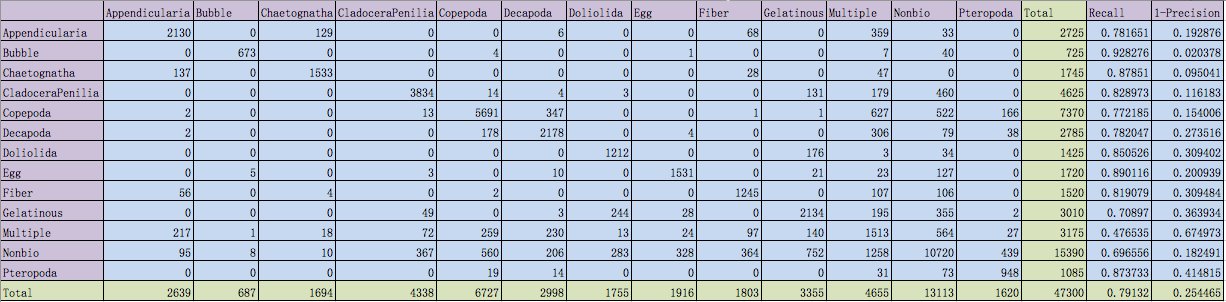
\includegraphics[width=1.0\linewidth]{19+7+LBP+IDSC-BF-FeatureFusion}
\caption{采用朴素贝叶斯分类器进行特征融合}
\label{fig:19+7+LBP+IDSC-BF-FeatureFusion}
\end{figure}

Bayesian Fusion of Color and Texture Segmentations, ICCV, 1999

A Study on Bayes Feature Fusion for Image Classification, CVPRW, 2003


\subsection{AdaBoost}
AdaBoost常用的弱分类器有:CART (classification and regression tree), decision stump, logistic regress等。AdaBoost最初设计用于解决二分类,对二分类问题,弱分类器条件要求对任意样本分布,分类器的分类准确率只需略高于 0.5,如果分类器过强容易产生过拟合。实际问题以多分类居多,AdaBoost在处理多分类问题时,对分类数目为$K$的多分类,要求弱分类器比随机猜测准确率$\frac{1}{K}$略高。

\subsubsection{尝试一(MATLAB中的AdaBoost)}
20个统计特征用AdaBoost算法进行分类,实验采用的MATLAB自带函数fitensemble,最大迭代次数设为50次,实现AdaBoost算法。实验结果如图\ref{fig:19+7-matlab-adaboost-50},分类准确率为63.1\%,低于随机森林得到的分类准确率73.7\%。
\begin{figure}[!ht]
\centering
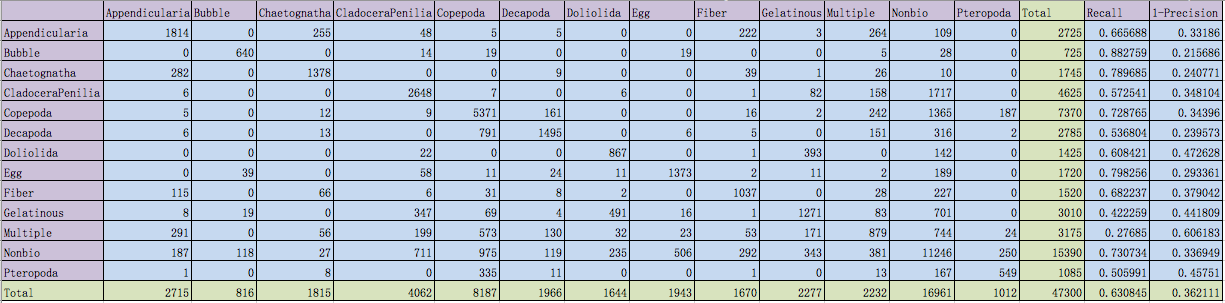
\includegraphics[width=1.0\linewidth]{19+7-matlab-adaboost-50}
\caption{20个特征采用MATLAB中的AdaBoost算法得到的分类结果}
\label{fig:19+7-matlab-adaboost-50}
\end{figure}

\subsubsection{尝试二(特征融合后采用AdaBoost)}
在特征融合方法一的基础上,将最终的分类方法SVM改为AdaBoost。实验结果如图\ref{fig:19+7+LBP+IDSC-Adaboost-FeatureFusion},分类准确率为70.9\%。
\begin{figure}[!ht]
\centering
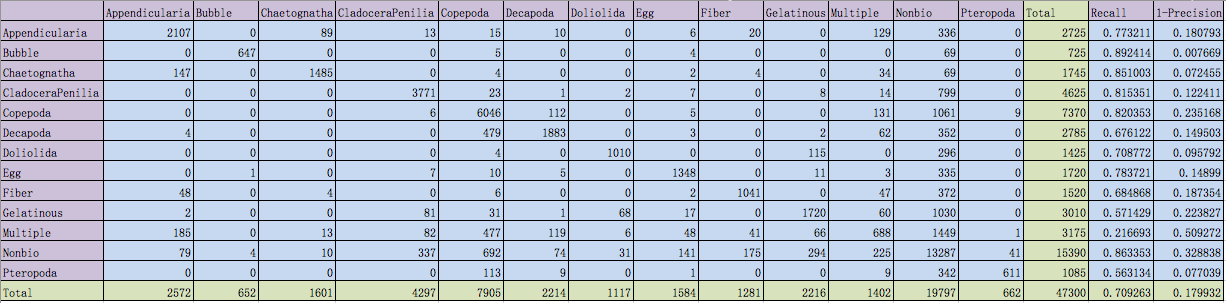
\includegraphics[width=1.0\linewidth]{19+7+LBP+IDSC-Adaboost-FeatureFusion}
\caption{采用Adaboost进行特征融合}
\label{fig:19+7+LBP+IDSC-Adaboost-FeatureFusion}
\end{figure}

\subsubsection{尝试三(将二分类改为多分类问题)}
代码:\url{https://code.google.com/p/adaboostmatlab/downloads/list}。

将解决二分类问题的算法改为解决多分类问题,采用拆分的方法。将多分类问题改成多个二分类问题,二分类为一对其余。实验结果如图\ref{fig:Adaboost+SVM-FeatureFusion},分类准确率为76.6\%。实验中遇到问题:
\begin{figure}[!ht]
\centering
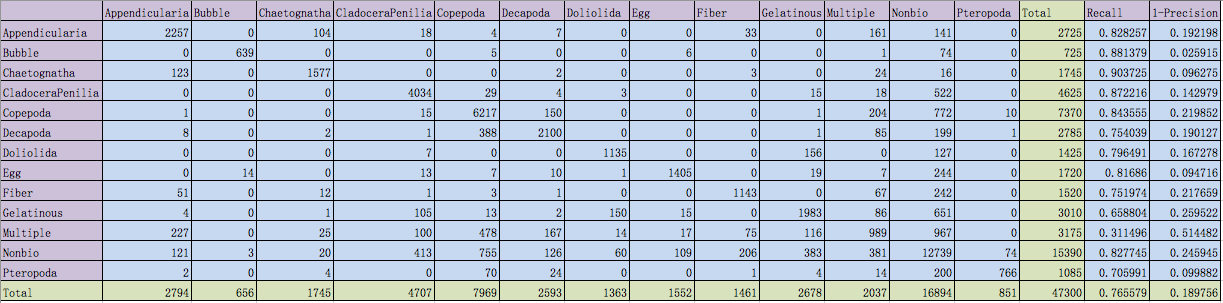
\includegraphics[width=1.0\linewidth]{Adaboost+SVM-FeatureFusion}
\caption{采用Adaboost+SVM进行特征融合}
\label{fig:Adaboost+SVM-FeatureFusion}
\end{figure}
\begin{itemize}
\item 实验中部分样本不能被识别(识别的结果13类都不是)。在实验中,我将这些不能识别的样本再用SVM进行分类。
\end{itemize}

\subsubsection{尝试四(将SVM作为弱分类器进行级联)}
该实验没有完成,在实现过程中发现两个问题:
\begin{itemize}
\item SVM作为弱分类器,在迭代的过程中不知道怎样输入样本权重。
\item 采用SVM根据已有的特征进行分类得到的分类结果已经超过50\%,这应该不是弱分类器,对它采用AdaBoost进行级联是不是会产生过拟合。
\end{itemize}



\subsubsection{AdaBoost应用}
AdaBoost可以用于:
\begin{enumerate}
\item 用于检测、识别和分类问题:AdaBoost应用最多的就是分类,通过级联弱分类器而得到强分类器,提高分类准确率。
\item 用于特征选择:在原始特征集合中,挑选出一些最具有代表性、可分性最好的特征子集。基于AdaBoost的特征选择过程:1、初始化训练样本权重 2、设计每个特征的分类器 3、根据加权训练样本最小错误率准则,选择分类器,也就是选择了特征 4、调整样本权重 5、通过循环,最后得到分类器的线性组合
\end{enumerate}
%近年来提出了对集成学习方法进行优化、剪枝。


\subsection{Multi-view Learning(多视角学习)}
周志华个人主页关于多视角学习:\url{http://cs.nju.edu.cn/zhouzh/zhouzh.files/publication/publication_toc.htm#Ensemble\%20Learning}。

多视角学习算法是Blum等\cite{blum1998combining}在用于半监督数据分类的联合学历算法中提出的。
多视角是指多个来源或多个特征子集。多视角学习算法有:
\begin{enumerate}
\item co-training(协同训练) :在未标记数据的两个不同视角下, 轮流的训练, 使相互一致性最大化。标准协同训练算法的步骤为:
    \begin{enumerate}
    \item 输入:标记数据集L,未标记数据集U。
    \item 用L1训练视图X1上的分类器f1,用L2训练视图X2上的分类器f2;
    \item 用f1和f2分别对未标记数据U进行分类;
    \item 把f1对U的分类结果中,前k个最置信的数据(正例p个反例n个)及其分类结果加入L2;把f2对U的分类结果中,前k个最置信的数据及其分类结果加入L1;把这2(p+n)个数据从U中移除;
    \item 重复上述过程,直到U为空集。
    \end{enumerate}
\item multiple kernel learning(多核学习):核指的是核函数。我们学过的SVM都是单核的,在使用的时候,需要根据经验或试验来选择用哪种核函数、怎样指定它的参数。然而实际对图像分类的实验中会用到纹理、形状等不同特征,这些特征最适合的核函数不一定相同,此时可以使用多核学习。多核学习:给定一些基本核函数,用它们的线性组合作为最终的核函数。通过训练得到线性组合中每一个核函数的权重。\footnote{\url{http://www.jianshu.com/p/ad010080a200}}
\item subspace learning(子空间学习):是指通过投影,实现高维特征向低维空间的映射,是一种经典的降维思想。
\end{enumerate}

\subsection{Fuzzy Neural Network}
代码:\url{http://www.mathworks.com/matlabcentral/fileexchange/4306-fuzzy-art-and-fuzzy-artmap-neural-networks}。

模糊神经网络是模糊理论和神经网络结合的产物,是具有模糊权系数或者输入信号是模糊量的神经网络。在特征融合方法一的基础上,将最终的分类方法 SVM 改为FNN,实验结果如图\ref{fig:19+7+LBP+IDSC-FNN-FeatureFusion},分类准确率为75.8\%。
\begin{figure}[!ht]
\centering
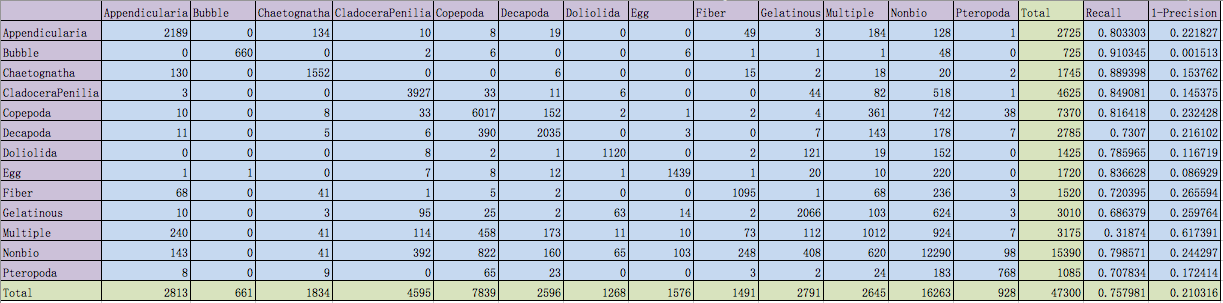
\includegraphics[width=1.0\linewidth]{19+7+LBP+IDSC-FNN-FeatureFusion}
\caption{采用FNN+SVM进行特征融合}
\label{fig:19+7+LBP+IDSC-FNN-FeatureFusion}
\end{figure}

Fuzzy neural networks: A survey, 1994


%\subsection{采用AdaBoost进行浮游动物分类}
%\subsubsection{尝试一}
%想要采用20个统计特征用AdaBoost级联的SVM将浮游动物分为13类,遇到的问题:
%\begin{itemize}
%\item AdaBoost常用于二分类问题,需要进行修改。
%\item 级联SVM产生的弱分类器,没有办法设置样本的权重。
%\end{itemize}
%
%\subsubsection{尝试二}
%采用AdaBoost在特征融合方法一的基础上,将最终的分类方法SVM改为AdaBoost。由于大多的AdaBoost都是处理二分类问题,因此该实验中将分为13类转换为13个二分类问题,实验结果如图\ref{fig:Adaboost+SVM-FeatureFusion},分类结果并没有提高。实验中遇到问题:
%\begin{figure}[!ht]
%\centering
%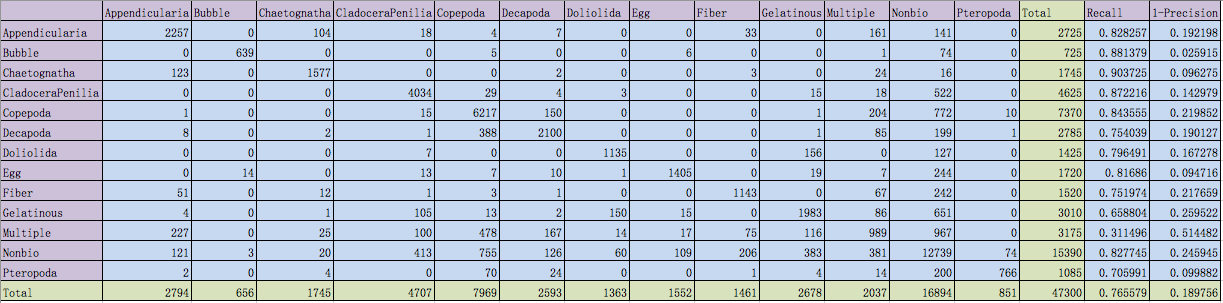
\includegraphics[width=1.0\linewidth]{Adaboost+SVM-FeatureFusion}
%\caption{采用Adaboost+SVM进行特征融合}
%\label{fig:Adaboost+SVM-FeatureFusion}
%\end{figure}
%\begin{itemize}
%\item 实验中部分样本不能被识别(识别的结果13类都不是)。在实验中,我将这些不能识别的样本再用SVM进行分类。
%\end{itemize}
%
%\subsubsection{尝试三}
%\textbf{模糊神经网络:}模糊神经网络就是模糊理论同神经网络相结合的产物,它汇集了神经网络与模糊理论的优点,集学习、联想、识别、信息处理于一体。模糊神经网络有如下三种形式:
%\begin{enumerate}
%\item 逻辑模糊神经网络
%\item 算术模糊神经网络
%\item 混合模糊神经网络
%\end{enumerate}

\bibliographystyle{plain}

\bibliography{Features} %参考文献